\chapter{Proposed solution}\label{ch:proposed-solution}
In chapter~\ref{ch:project-problem}, the problem that this project aims to address was outlined along with a short
description of the proposed solution. This chapter builds upon that giving a format mathematical model for the problem
(section~\ref{sec:optimisation-problem}). While the overall problem is about resource allocation,servers
would wish to be paid for the use of their resource so section~\ref{sec:auctioning-of-tasks} addresses this by proposing
an auction mechanism for tasks. Using the optimisation problem and auction mechanism from the previous sctions,
agents for both the auction and to allocate resources are proposed in section~\ref{sec:proposed-agents} that learn to
together to maximise servers profits over time.

\section{Resource allocation optimisation problem}\label{sec:optimisation-problem}
Using the flexible resource principle that the time taken for a operation to
occur, e.g.\ loading of a program, computing the program and sending of results, etc, is proportional to the amount of
resources allocated to completed the operation. A modified version of a resource allocation optimisation model can be
formatted by building upon a similar formulation in~\cite{FlexibleResourceAllocation}.

A sketch of the whole system is shown in figure~\ref{fig:system_model}.
The system is assumed to contain a set of $I = \{1,2,\ldots,\left|I\right|\}$ servers that are heterogeneous in all
characteristics. Each server has a fixed resources capacity: storage for the code/data needed to run a task
(e.g., measured in GB), computation capacity in terms of CPU cycles per time interval (e.g., measured in FLOP/s),
and communication bandwidth to receive the data and to send back the results of the task after execution
(e.g., measured in Mbit/s). The resources for server $i$ are denoted: $S_i$ for storage capacity, $W_i$ for computation
capacity, and $R_i$ for communication capacity.

\begin{figure}[h]
    \centering
    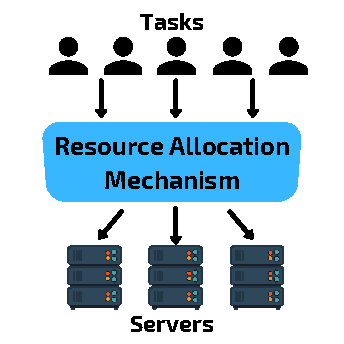
\includegraphics[width=8cm]{figures/system_model.pdf}
    \caption{System model}
    \label{fig:system_model}
\end{figure}

The system is also assumed to contain a set of $J = \{1,2,\ldots,\left| J \right|\}$ heterogeneous tasks that require
service from one of the servers in set $I$. To run any of these tasks on a server requires storing the appropriate
code/data on the same server. This could be, for example, a set of images, videos or convolutional neural network
layers in identification
tasks. The storage size of task $j$ is denoted as $s_j$ with the rate at which the program is transferred to the server
$i$ at time $t$ being $s^{'}_{j,t}$. For a task to be computed successfully, it must fetch and execute instructions
on a CPU. We consider the total number of CPU cycles required for the program to be $w_j$, where the number of
CPU cycles assigned to the task on server $i$ at time $t$ is $w^{'}_{j,t}$. Finally, after the task is run and
the results obtained, the latter need to be sent back to the user. The size of the results for task $j$ is denoted with
$r_j$, and the rate at which they are sent back to the user is $r^{'}_{j,t}$ on server $i$ at time $t$. Every task
has an auction time, denoted by $a_j$ and a deadline, denoted by $d_j$. This is the time step when the task is auctioned
and the last time for which the task can be completed successful at.
During this time, the time required to send the data/code to the server, run it on the server, and get back the results
to the user which must occur in order. As a server couldn't start computing a task that was already fully loaded on the
machine, for example.

Because of this, three additional variables are required for track the progress of each task stage.
$\hat{s}_{j,t}$ denotes the loading progress of the task, $\hat{w}_{j,t}$ denotes the compute progress and
$\hat{r}_{j,t}$ denotes the sending progress of the task. Each of these variables are updated recursively depending
on the progress in the previous time step plus the resources allocated.

\begin{align}
    \hat{s}_{j,t+1} = \hat{s}_{j,t} + s^{'}_{j,t} & \forall {j \in J, t \in T } \label{eq:loading_progress} \\
    \hat{w}_{j,t+1} = \hat{w}_{j,t} + w^{'}_{j,t} & \forall {j \in J, t \in T } \label{eq:compute_progress} \\
    \hat{r}_{j,t+1} = \hat{r}_{j,t} + r^{'}_{j,t} & \forall {j \in J, t \in T } \label{eq:sending_progress} \\
\end{align}

% TODO
% Add more constraints
% Add sentence on time
% Add deadline constraint with explanation

As server have limited capacity, the total resource usages for all tasks running on a server must be capped.
The storage constraint (equation~\eqref{eq:server_storage_capacity}) is unique it the sum of the loading progress for
each task allocated to the server. While the computation capacity
(equation~\eqref{eq:server_computation_capacity} is the sum of compute used by all of the tasks on a server $i$ at
time $t$ and the bandwidth capacity (equation~\eqref{eq:server_bandwidth_capacity}) is the sum of loading and sending
usages by tasks.

\begin{align}
    \sum_{j \in J} \hat{s}_{j,t} x_{i,j} \leq S_i, && \forall{i \in I, t \in T} \label{eq:server_storage_capacity} \\
    \sum_{j \in J} w^{'}_{j,t} x_{i,j} \leq W_i, && \forall{i \in I, t \in T} \label{eq:server_computation_capacity} \\
    \sum_{j \in J} (s^{'}_{j,t} + r^{'}_{j,t}) x_{i,j} \leq R_i, && \forall{i \in I, t \in T} \label{eq:server_bandwidth_capacity} \\
\end{align}

\section{Auctioning of Tasks}\label{sec:auctioning-of-tasks}
While the mathematically description of the problem presented in the previous section doesn't consider any auctions
occurring. In real
life services normally wish to be paid to the use of their resources. However due to the modifications that
this project has to make to the optimisation problems. All of the auction mechanisms discussed in section~\ref{sec:related-work-in-cloud-computing} cannot
be used. This is primarily as the user is not requesting a fixed amount of resources nor can the available resources be easily computed
as this is dynamic depending on the stages of tasks allocated to a server. Also the algorithms presented in ~\cite{FlexibleResourceAllocation}
assume that all of the task stages can occur concurrently, an idea this optimisation prevents. This means that a novel or modified auction
mechanism must be used to deal with these changes. Due to the complexities of devising new auction mechanism and the
large corpus of research on auctions already, this project choose to use the Vickrey auction~\citep{vickrey}.

But a modification must be made as servers generate the prices for tasks rather than task suggesting a price to servers.
Because of this auction is reversed, such that the servers with the minimum price wins the task instead of the maximum
price. The auction therefore works by allowing all servers to submit their bids for a task with the winner being the
server with the lowest price but task actually pays second lowest price. The reason this auction was selected over
alternatives is explained in section~\ref{sec:justification-of-auction-mechanisms}.

\section{Proposed Agents}\label{sec:proposed-agents}
Using the optimisation formulation and auction problem from the previous two sections, the problem can modelled as
Markov Decision Process~\cite{Bel} which allows the environment to be format like in figure~\ref{fig:mdp_system_model}.
This separates out the auction and resource allocation part of the problem with separate agents to act during their
respective part of the problem. Subsection~\ref{subsec:proposed-auction-agents}
and~\ref{subsec:proposed-resource-allocation-agents} proposed agents for the auction environment and resource allocation
environment respectively.

\begin{figure}
    \centering
    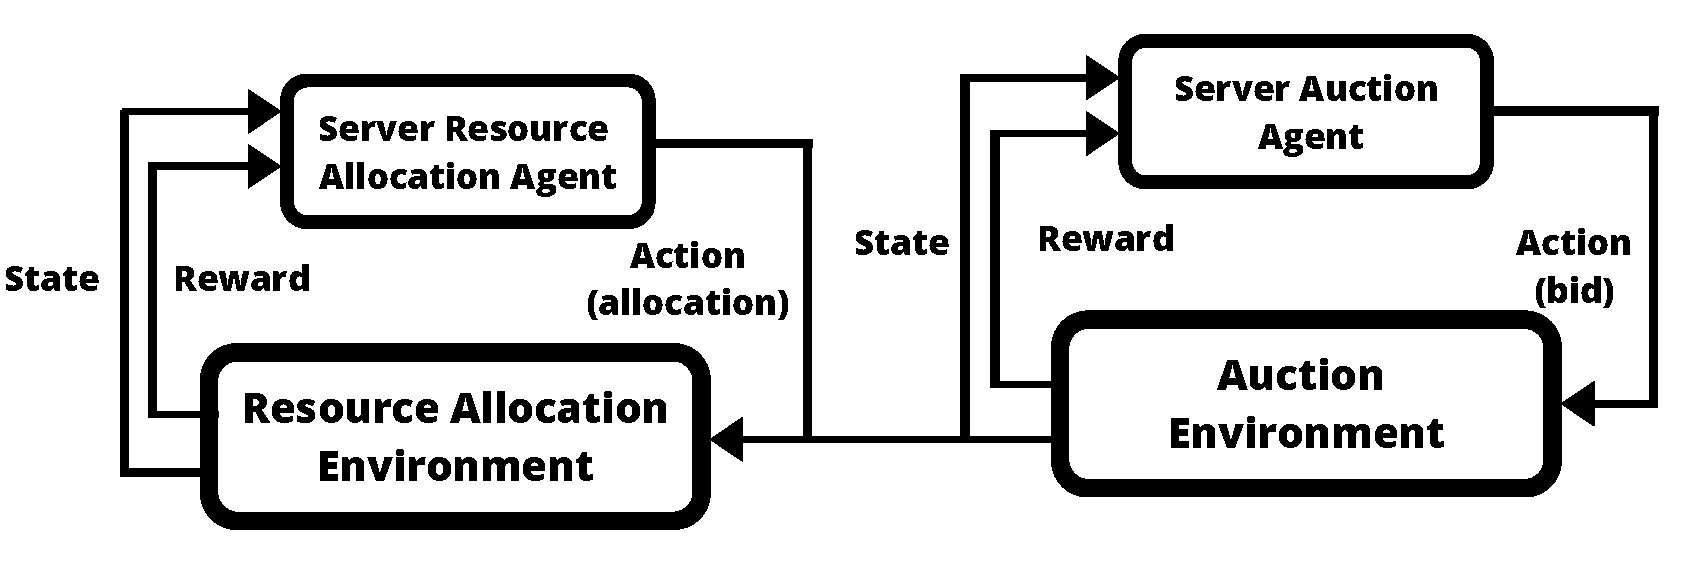
\includegraphics[width=14cm]{figures/flexible_resource_allocation_env.pdf}
    \caption{Markov Decision process system model}
    \label{fig:mdp_system_model}
\end{figure}

The environment is believed to of particularly interest for multi-agent reinforcement learning researchers as the aim
of the environment is cooperative (to maximise the social welfare) but knowing that servers acts self-interestedly in
competition during the auctions in order to maximise their private profits. But the resource allocation agent must work
cooperatively in allocating of resources for each task as the server wishes to complete as many tasks as they can.

\subsection{Proposed auction agents}\label{subsec:proposed-auction-agents}
Traditionally pricing mechanisms~\citep{al2013cloud} rely on mixture of metrics; resource availability, resource demand,
quality of service, task resource requirements, task resource allocation quantity, etc to determine a price. However
these values are difficult to approximate during the auction. Due to the complexity of deriving this function,
Reinforcement Learning will be used with the aim to learn an optimal policy to maximise the profits of the server.
Simple heuristics will also be implemented in order compare the effectiveness of the reinforcement learning to
untrained heuristics.

As the action space of the agent is continuous, a deep deterministic policy gradient~\citep{ddpg} agent that allows
will be implemented. The action shape can also be discretized allow deep Q learning agents~\cite{atari} to be trained
as well. In order to compare alternative learning methods and the affect of discretizing the action space on results.

These agents will use neural networks to learn as it is known to be able to approximate any function
~\citep{csaji2001approximation}.
Because of this, a long/short term memory~\citep{LSTM} layer will be used as it allows for multiple inputs, and outputs
are single vector that will have several additional layers to allow additional complexity.
The network ending at a single ReLU neuron for DDPG or multiple logit activation neurons for DQN agents. The
justification for this network over other neural network models is explained in
section~\ref{subsec:justification-for-auctioning-networks}.

% Todo add image of proposed network

\subsection{Proposed resource allocation agents}\label{subsec:proposed-resource-allocation-agents}
When a new task is allocated to the server or a task completes a stage then the server resource need to be
redistributed. As the problem of how to allocation resources isn't as complex as the agent pricing in
section~\ref{subsec:proposed-auction-agents}, both simple heuristics and reinforcement learning agents will be
implemented in order to compare effectiveness.

However a similar problem exists to the proposed auction agents (in subsection~\ref{subsec:proposed-auction-agents}) as
to know how to allocate resources to be single task while being aware of the resource requirements of other tasks that
the server has allocated. Therefore a similar network is proposed to allow for the other tasks to be passed in in order
to compare the current task having resources allocated to and the other tasks also allocated to the server.

A weighting heuristic is therefore proposed where the exact resources for the task are determined by tinstead a weighted version.
This has the advantage of being a simpler function to approximated for agents with a similar expresssiveness as a
true allocation function. While avoiding the problem of over allocating the resources.
